\documentclass[11pt, a4paper, twoside]{article}   	% use "amsart" instead of "article" for AMSLaTeX format

\usepackage{geometry}                		% See geometry.pdf to learn the layout options. There are lots.
\usepackage{pdfpages}
\usepackage{caption}
\usepackage{minted}
\usepackage[german]{babel}			% this end the next are needed for german umlaute
\usepackage[utf8]{inputenc}
\usepackage{color}
\usepackage{graphicx}
\usepackage{titlesec}
\usepackage{fancyhdr}
\usepackage{lastpage}
\usepackage{hyperref}
% http://www.artofproblemsolving.com/wiki/index.php/LaTeX:Symbols#Operators
% =============================================
% Layout & Colors
% =============================================
\geometry{
   a4paper,
   total={210mm,297mm},
   left=20mm,
   right=20mm,
   top=20mm,
   bottom=30mm
 }	

\definecolor{myred}{rgb}{0.8,0,0}
\definecolor{mygreen}{rgb}{0,0.6,0}
\definecolor{mygray}{rgb}{0.5,0.5,0.5}
\definecolor{mymauve}{rgb}{0.58,0,0.82}

\setcounter{secnumdepth}{4}


% the default java directory structure and the main packages
\newcommand{\suiteMainSrcDir}{../../junit-test-suite/src/main/java/at/fh/ooe/swe4/junit/test/suite/watcher}
\newcommand{\srcDir}{../src/main/java}
\newcommand{\srcTestDir}{../src/test/java}
\newcommand{\resourcesTestDir}{../src/test/resources}
\newcommand{\mainPackageDir}{\srcDir/at/fh/ooe/swe4/puzzle}
\newcommand{\mainTestPackageDir}{\srcTestDir/at/fh/ooe/swe/test}
\newcommand{\boardTestPackageDir}{\mainTestPackageDir/puzzle/impl/boardImpl}
\newcommand{\searchNodeTestPackageDir}{\mainTestPackageDir/puzzle/model/searchNode}
\newcommand{\sliderTestPackageDir}{\mainTestPackageDir/puzzle/impl/slidingPuzzle}
\newcommand{\mainTestPackage}{at.fh.ooe.swe.test}
\newcommand{\imagesDir}{images}
% the default subsection headers
\newcommand{\ideaSection}{Lösungsidee}
\newcommand{\sourceSection}{Source-Code}
\newcommand{\testSection}{Tests}

% =============================================
% Code Settings
% =============================================
\newenvironment{code}{\captionsetup{type=listing}}{}
\newmintedfile[javaSourceFile]{java}{
	linenos=true, 
	frame=single, 
	breaklines=true, 
	tabsize=2,
	numbersep=5pt,
	xleftmargin=10pt,
	baselinestretch=1,
	fontsize=\footnotesize
}
\newmintinline[inlineJava]{java}{}
\newminted[javaSource]{java}{
	breaklines=true, 
	tabsize=2,
	autogobble=true,
	breakautoindent=false
}
\newmintedfile[xmlSourceFile]{xml}{
	linenos=true, 
	frame=single, 
	breaklines=true, 
	tabsize=2,
	numbersep=5pt,
	xleftmargin=10pt,
	baselinestretch=1,
	fontsize=\footnotesize
}
\newmintedfile[propertiesFile]{properties}{
	linenos=true, 
	frame=single, 
	breaklines=true, 
	tabsize=2,
	numbersep=5pt,
	xleftmargin=10pt,
	baselinestretch=1,
	fontsize=\footnotesize
}
% =============================================
% Page Style, Footers & Headers, Title
% =============================================
\title{Übung 3}
\author{Thomas Herzog}

\lhead{Übung 3}
\chead{}
\rhead{
\includegraphics[scale=0.10]{FHO_Logo_Students.jpg}}

\lfoot{S1310307011}
\cfoot{}
\rfoot{ \thepage / \pageref{LastPage} }
\renewcommand{\footrulewidth}{0.4pt}
% =============================================
% D O C U M E N T     C O N T E N T
% =============================================
\pagestyle{fancy}
\begin{document}
\setlength{\headheight}{15mm}
\includepdf[pages={1-4}]{Swe4xA04_BB_2.pdf}
{\color{myred}
	\section
		{Verschiebe Puzzle A*-Algorithmus}
}

\subsection{\ideaSection}
Folgend ist die Dokumentation für die Aufgabenstellung Verschiebe Puzzle mit dem A*-Algorithmus lösen angeführt. \\
Es werden zwar Klassenspezifikationen vorgegeben, jedoch soll nicht stur diesen gefolgt werden, obwohl die Semantik beibehalten werden soll.\\
Bezüglich der konkreten Spezifikation der APIs und Implementierungen sei auf den Bereich \emph{Source} verwiesen, wo einerseits beschrieben wird warum die API oder Implementierung so gewählt wurde und andererseits ist im angeführten Source die Javadoc enthalten. Ich finde es besser den Source über Javadoc zu kommentieren als in einem externen Dokument.

\subsubsection{Maven Projekt}
Dieses Mal soll das Projekt als Maven Projekt implementiert werden, da es sich hierbei um ein bekanntes und meist genutztes Framework für Build Konfiguration handelt und es sehr einfach erlaubt Dependencies einzubinden und auch automatisch die Sources dieser Dependencies zur Verfügung stellt.\\
Dies sollte kein Problem darstellen, da Eclipse LUNA bereits mit Maven ausgeliefert wird. Es soll gewährleistet werden, dass es keine speziellen Konfigurationen erfordert um das Projekt zu importieren und es zum Laufen zu bringen.\\
Jedoch sei angemerkt das ein \emph{Update Projekt} von Nöten sein wird um alle Dependencies von den Maven Repositories zu laden. Des Weiteren sollen keine Änderungen an der Standard \emph{settings.xml} vorgenommen werden.\\\\
Für weitere Informationen bezüglich der Maven Konfiguration sei auf den Bereich \emph{Projekt Konfiguration} verwiesen, in dem die \emph{pom.xml} angeführt ist. Dort ist auch beschrieben mit welchen Maven Build command das Projekt gebuildet werden soll, da es auch Konfigurationen geben soll, die einen report für die Tests erstellen. 

\subsubsection{JUnit Tests}
Wie verlangt soll testgetrieben vorgegangen werden wobei anstatt einer riesigen Testklasse je getesteter Methode eine eigene Testklasse implementiert werden soll.\\
So sind Tests übersichtlicher und es kann auch keinen Namenskonflikte geben. Des Weiteren wird es pro getesteter Methode sicherlich mehr als eine Testmethode geben. \\
Bei den JUnit Tests soll sich an folgende Konvention gehalten werden: \\
\begin{enumerate}
	\item \textbf{Root Package:} Alle Test-Klassen sollen im package \emph{\mainTestPackage.*} zusammengefasst werden. Dadurch liegen alle Testklassen in einer eignen Domain und sind völlig unabhängig vom dem eigentlichen Source
	\item \textbf{API-Package:} Alle Test Ressourcen wie z.B.: abstrakte Testklassen sollen im Package \emph{\mainTestPackage.api.*} liegen. Dadurch ist erkennbar das es sich hierbei um eine API für die Tests handelt des getesteten Projektes handelt.
	\item \textbf{Test Packages:} Alle tatsächlichen Tests sollen in Packages liegen die wie folgt aufgebaut sein sollen '\emph{\mainTestPackage.\textless sourcePackage\textgreater .\textless testedClassName\textgreater (\mainTestPackage.puzzle.impl.boardImpl.*)}', wobei man sich an die Java Bean Convention zu halten hat.
	\item \textbf{Test-Klassen:} Die Test-Klassen Name sollen wie folgt aufgebaut sein: '\emph{\textless testedMethodName\textgreater Test (SolveTest, MakeMoveTest, usw.)}'. Ein Spezialfall könnten die Klassen sein, die zur Verfügung gestellt worden, wenn diese in Konflikt mit bestehenden Testklassen stehen.
	\item \textbf{Test-Methoden:} Die Testmethoden sollen so benannt werden, dass man leicht erkennen kann was getestet wird. Ein Präfix mit \emph{test} ist zu vermeiden, da ja klar ist das es sich bei Methoden in Testklassen um Tests handelt. \emph{(nullIterable, validAllFieldsRowPerRowLeftToRight, usw.)}
\end{enumerate}
Für die JUnit Test soll JUnit4 verwendet werden wobei hierbei so viele Features wie möglich genutzt werden sollen. Da sicherlich bei den nächsten Übungen auch JUnit Test implementiert werden müssen, sollen alle Ressourcen, die bei anderen Tests wiederverwendet werden können in ein eigenes Projekt ausgelagert werden \emph{junit-test-suite}, sodass diese Ressourcen einfach in anderen Projekten verwendet werden können. Es ist darauf zu achten, dass es absolut keine Abhängigkeiten zu dem eigentlichen Projekt gibt und das die Implementierungen so aufgebaut sind, dass sie für jedes anderes Projekt ohne Modifikation wiederverwendet werden können. \\\\
Da wir dazu gezwungen sind in dieser Dokumentation auch die Testresultate anzuführen und die Screenshots von JUnit im Eclipse zu wenig erscheinen, soll ein Logging implementiert werden, dass die Testresultate auf der Konsole ausgibt. Hierbei sollen \emph{TestWatcher} implementiert werden, die einerseits die Invocation einer Testklasse sowie andererseits die Invocation einer Testmethode auf die Konsole loggen. Hierbei soll ein bekanntes Logging Framework namens Log4j verwendet werden.

\subsection{A*-Algorithmus}
Da der A*-Algorithmus bei dieser Problemstellung eine riesige Lösungsmenge produziert könnte, muss dieser optimiert werden.\\
Pro untersuchten Knoten können maximal 4 Nachfolgeknoten gefunden werden, was bedeutet, dass im schlimmsten Fall pro untersuchter Ebene der Lösungsbaum um den Faktor 4 anwächst.\\\\
Folgend ist ein Beispiel für den worst case angeführt wobei \emph{M} die zu untersuchende Lösungsmenge darstellt:
\begin{enumerate}
	\item $M=\{N1\}$
	\item $M=\{N1, N2, N3, N4, N5\}$
	\item $M=\{N1, N2, N3, N4, N5, N6, N7, N8, N9\}$
	\item ...
\end{enumerate}
Es ist zu sehen dass bereits bei der dritten Ebene sich 9 Elemente in der zu untersuchenden Lösungsmenge befinden. Daher muss der Algorithmus so optimiert werden, wobei die noch nicht untersuchten Knoten (offen Knoten) und die bereits untersuchten Knoten (geschlossene Knoten) geprüft werden müssen ob bereits Knoten untersucht wurden, die geringere Kosten aufweisen. Ist dem so, dann soll der Nachfolgeknoten mit den höheren Kosten von der Untersuchung ausgeschlossen werden, was die Lösungsmenge so klein wie möglich hält.\\
Hierbei stellen aber die Implementierungen \inlineJava{node.hashCode(); node.equals(Object other)} der Klasse \inlineJava{SearchNode<T>} ein Problem dar, da aufgrund der verwendeten \inlineJava{PriorityQueue<T>} diese Methoden die Kosten mit aufnehmen müssen.\\
Ansonsten würden bei dem Versuch Knoten aus der Queue zu löschen alle Knoten gelöscht werden, die dasselbe Board halten aber unterschiedliche Kosten.\\
Des Weiteren macht es dieser Umstand unmöglich einen Knoten mit einem bestimmten gesetzten Board zu erhalten, da ja auch die Kosten mit involviert sind.\\
Eine Verwendung des Containers \inlineJava{Set<T>, List<T>} scheidet ebenfalls aus da wir bei der untersuchung der offenen und geschlossenen Knoten Knoten erhalten müssen, die lediglich dasselbe \inlineJava{Board<T>} halten ohne Rücksicht auf deren Kosten. \\\\
Daher wurden folgende Container gewählt:\
\begin{enumerate}
	\item \textbf{\inlineJava{PriorityQueue<T>}:} Die Queue, die die Knoten mit den geringsten Kosten vorne anreiht und diese zuerst zurückliefert. Erfordert bei \inlineJava{node.hashCode(); node.equals(Object other)} die Miteinbeziehung der Kosten.
	\item \textbf{\inlineJava{HashMap<Board<T>, SearchNode<T>>}: } Für die bereits untersuchten und offenen Knoten. Hierbei haben wir konstante Laufzeit beim Hinzufügen und Erhalten eines Knoten aus der Map, da hier über die Hashfunktion \inlineJava{board.hashCode()} die Knoten in der Map adressiert werden. Ebenfalls wird so das Problem mit \inlineJava{node.hashCode(); node.equals(Object other)} umgangen. (Beinahe konstante Laufzeit aufgrund von Kollisionen) 
\end{enumerate}
Der Algorithmus soll versuchen die Nachfolgeknoten des aktuell untersuchten Knoten in den Container, offene wie auch geschlossenen Knoten, zu finden und zu entscheiden ob diese Knoten des Containers geringere Kosten besitzen. Wenn ja werden die aktuellen Nachfolgeknoten ignoriert und nicht weiter untersucht, da es schon einen besseren Weg zu diesem Board gibt.

\newpage
\subsection{Project Konfigurationen}
Folgend sind die Projektkonfigurationen angeführt wie \emph{pom.xml} und \emph{log4j.properties}.\\
Wenn das Projekt in Eclipse importiert wird, so muss zuerst ein \emph{Update Project} über das Kontextmenu des Projekts \emph{\textless maven\_project\textgreater - Maven - Update Project} gemacht werden, damit die Dependencies in das lokale Maven Reporsitory geladen werden.\\
Danach kann das Projekt mit folgenden maven-build command gebuildet werden:\\
\emph{clean test-compile surefire-report:report site}
\begin{enumerate}
	\item \textbf{clean:} Löscht Inhalt des Verzeichnisses \emph{\$\{basedir\}/target}
	\item \textbf{test-compile:} Kompiliert, testet und packaged das Projekt in das Verzeichnis \emph{\$\{basedir\}target}
	\item \textbf{surefire-report:resport:} Erstellt den Surefire Report in dem Verzeichnis \emph{\$\{basedir\}/target/surefire-reports}
	\item \textbf{site:} Erstellt einen Maven Report in dem Verzeichnis \emph{\$\{basedir\}/target/site} mit allen Projektinformationen und beinhaltet auch die Surefire Reports
\end{enumerate}
Ebenfalls wird \emph{log4j} als Logging Framework verwendet und diese Framework benötigt eine Konfiguration für die verwendeten Logger.\\
Da die Logger nur für die Tests verwendet werden, ist sie im Verzeichnis \emph{\$\{basedir\}/src/test/resources} enthalten und nicht in \emph{\$\{basedir\}/src/main/resources} .\\

\subsubsection{pom.xml}
Folgend ist die \emph{pom.xml} des Projekts angeführt.\\
Es wird hierbei das \emph{maven-compiler-plugin} und \emph{maven-surefire-plugin} verwendet. Letzteres wird dazu verwendet um den Test Report zu erstellen.
\begin{code}
	\caption{pom.xml}
	\xmlSourceFile{../pom.xml}
\end{code}
\subsubsection{log4j.properties}
Folgend ist die \emph{log4j.properties} des Projekts angeführt.\\
Hier sind die Logging Konfigurationen für \emph{log4j} enthalten.
\begin{code}
	\caption{log4j.properties}
	\propertiesFile{\resourcesTestDir/log4j.properties}
\end{code}
\newpage

\subsection{JUnit Testsuite Source}
Folgend sind die Sources der JUnit Testsuite angeführt.

\subsubsection{AbstractLoggerWatcher.java}
Diese Klasse dient als Basis für die LoggerWatcher und kapselt alle gemeinsamen Konfigurationen und Ressourcen.
\begin{code}
	\caption{AbstractLoggerWatcher.java}
	\javaSourceFile{\suiteMainSrcDir/api/AbstractLoggerWatcher.java}
\end{code}
\newpage

\subsubsection{LoggingTestClassWatcher.java}
Diese Klasse logt die Invocation einer Testklasse.
\begin{code}
	\caption{LoggingTestClassWatcher.java}
	\javaSourceFile{\suiteMainSrcDir/LoggingTestClassWatcher.java}
\end{code}
\newpage

\subsubsection{LoggingTestInvocationWatcher.java}
Diese Klasse logt die Invocation einer Testmethode.
\begin{code}
	\caption{LoggingTestInvocationWatcher.java}
	\javaSourceFile{\suiteMainSrcDir/LoggingTestInvocationWatcher.java}
\end{code}
\newpage

\subsection{N-Puzzle Source}
Folgend sind die Sources des n-puzzle-problem Projekts angeführt.

\subsubsection{BoardListImpl.java}
Folgend ist das Interface \emph{Board<T extends Comparable<T>>} angeführt, welches die Spezifikation für die Board Implementierung darstellt. Es wurde beschlossen ein eigenes Interface zu spezifizieren, da es auch möglich sein soll den Container für die Verwaltung der Kacheln auszutauschen (\inlineJava{List<T>, T[], usw.})\\
Des weiteren wurde beschlossen eine Typdefinition zu verlangen, da es auch möglich sein soll andere Datentypen außer Integer für die Kacheln zu verwenden. Die einzige Voraussetzung dafür ist, dass sich der Datentyp einer Rangordnung unterwerfen lässt, was über das Interface \inlineJava{Comparable<T>} gewährleistet wird. Es spielt hierbei keine Rolle um welchen Datentyp es sich handelt \inlineJava{Integer, BigInteger, Decimal, Character, usw.}, das einzig wichtige ist das der Datentyp das Interface \inlineJava{Comparable<T>} korrekt implementiert.    
\begin{code}
	\caption{BoardListImpl.java}
	\javaSourceFile{\mainPackageDir/api/Board.java}
\end{code}
\newpage

\subsubsection{BoardImpl.java}
Folgend ist die Implementierung für das Interface \inlineJava{Board<T extends Comparable<T>>} angeführt, welches als Container eine \inlineJava{ArrayList<T>} verwendet. Dieser Container wurde gewählt da es sich im Hintergrund um ein \inlineJava{Object[]} handelt, daher indexierte Zugriffe möglich sind und dieser Container Methoden zur Verfügung stellt, die den Zugriff bzw. die Handhabung dieses \inlineJava{Object[]} erleichtern.\\
Der Container wird mit der zu erwartenden Größe initialisiert um ein dynamisches wachsen, welches ein \inlineJava{Array.copy(...)} verursacht, zu vermeiden.\\
Dies ist zwar nicht zwingend notwendig aber ist als Best Practise anzusehen.
\begin{code}
	\caption{Board.java}
	\javaSourceFile{\mainPackageDir/impl/BoardListImpl.java}
\end{code}
\newpage

\subsubsection{SlidingPuzzle.java}
Folgend ist die Implementierung des \inlineJava{SlidingPuzzle<T extends Comparable<T>>} angeführt, welches die Boards versucht in die Zielkonfiguration zu überführen. Da es möglich sein soll nicht ur eine Zielkonfiguration zu handhaben wurde die Implementierung erweitert um die Möglichkeit eine Zielkonfiguration zu übergeben.\\
Diese Klasse wurde mit dem Pattern \emph{Fluent Interface} implementiert, da es dieser Pattern erlaubt hier eine gut verständliche Aufrufkette aufzubauen. Diese Aufrufkette liest sich wie Prosa wie in diesem Beispiel ersichtlich. 
\begin{javaSource}
	// Create new slide instance
	SlidingPuzzle<Integer> slider = new SlidingPuzzle<>(); 
	// start the slider with the initial board
	slider.start(initialBoard)
		// Try to solve the board (returns SolutionHandler instance)
		.solve(goalBoard)      
		// Starts the SolutionHandler instance
		.start()      
		// Regsiter custom logger with custom level
		.registerLogger(myLog, Level.DEBUG)   
		// Fill resulting moves in given list      
		.fillMoves(moves)
		// prints the resulting moves via the logger
		.printMoves()
		// performs the moves on the inital board and logs inital/resulting board state
		.performMoves()
		// ends the SolutionHandler, returns related SlidingPuzzle instance
		.end()
		// Ends the SlidingPuzzle instance (reset state)
		.end();
\end{javaSource} 
Es wurde eine interne Klasse \inlineJava{SolutionHandler<T extends Comparable<T>>} implementiert, welche das Handling der Lösung übernimmt. Auch diese Implementierung verwendet \emph{Fluent Interface}. \\
Um durchgehend mit demselben Typ zu arbeiten zu können wird auch hier die Typdefinition verlangt, die der Typdefinition der Kacheln im \inlineJava{Board<T extends Comparable<T>>} entspricht. Damit ist gewährleistet, dass z.B.: eine \inlineJava{SlidingPuzzle<Integer>} Instanz nur auf \inlineJava{Board<Integer>} Instanzen angewendet werden kann und nicht z.B.: auf \inlineJava{Board<Character>} Instanzen.\\\\
\begin{code}
	\caption{BoardListImpl.java}
	\javaSourceFile{\mainPackageDir/impl/SlidingPuzzle.java}
\end{code}
\newpage

\subsubsection{Position.java}
Folgend ist der Source des Models \inlineJava{Position} angeführt, welches dafür verwendet wird um die Position der leeren Kacheln zu liefern, da es mir zu wenig erschien nur mit der Spalte der leeren Kacheln zu arbeiten.
\begin{code}
	\caption{Position.java}
	\javaSourceFile{\mainPackageDir/model/Position.java}
\end{code}
\newpage

\subsubsection{SearchNode.java}
Folgend ist der Source des Models \inlineJava{SearchNode<T extends Comparable<T>>} angeführt, welches den Knoten für den A*-Algorithmus darstellt. Hierbei sei die Implementierung der Methoden \inlineJava{node.hashCode(); node.equals(other)} erwähnt, die nicht nur das referenzierte \inlineJava{Board<T>} verwendet sondern auch die Gesamtkosten.\\
Das Problem mit diesen Implementierungen ist, dass bei der Verwendung eines \inlineJava{Set<T>} Containers, welcher die geschlossenen Knoten enthält, Duplikate enthalten würde. Also Knoten mit demselben \inlineJava{Board} aber mit unterschiedlichen gesetzten Kosten.\\
Daher dürfen diese offenen und geschlossenen Knoten nicht in Containern verwendet werden, die deren \inlineJava{node.hashCode(); node.equals(Object other)} verwenden.
\begin{code}
	\caption{SearchNode.java}
	\javaSourceFile{\mainPackageDir/model/SearchNode.java}
\end{code}
\newpage

\subsection{N-Puzzle Exception Source}
Folgend ist der Source der implementierten Exceptions angeführt.

\subsubsection{InvalidBoardIndexException.java}
Folgend ist die Implementierung der \inlineJava{InvalidBoardIndexException extends RuntimeException} angeführt, welche verwendet wird um anzuzeigen das ungültige Indizes gefunden wurden.
\begin{code}
	\caption{InvalidCoardIndexException.java}
	\javaSourceFile{\mainPackageDir/exception/InvalidBoardIndexException.java}
\end{code}

\subsubsection{InvalidMoveException.java}
Folgend ist die Implementierung der \inlineJava{InvalidMoveException extends RuntimeException} angeführt, welche verwendet wird um anzuzeigen wenn versucht wurde die leere Kachel auf eine ungültige Position zu verschieben.
\begin{code}
	\caption{InvalidMoveException.java}
	\javaSourceFile{\mainPackageDir/exception/InvalidMoveException.java}
\end{code}

\subsubsection{NoSolutionExcption.java}
Folgend ist die Implementierung der \inlineJava{NoSolutionExcption extends Exception} angeführt, welche verwendet wird um anzuzeigen das keine Lösung gefunden wurde. Diese Ausnahme muss explizit abgefangen werden.
\begin{code}
	\caption{NoSolutionExcption.java}
	\javaSourceFile{\mainPackageDir/exception/NoSolutionExcption.java}
\end{code}
\newpage

\subsection{N-Puzzle Test Source}
Folgend ist der Source der N-Puzzle Tests angeführt.

\subsubsection{AbstractTest.java}
Folgend ist die Implementierung der abstrakten Testklasse angeführt, welche die gemeinsamen Ressourcen für die konkreten Testklassen kapselt.\\
Hier sind \inlineJava{TestWatcher} deklariert, die das Logging der Tests realisieren.
\begin{code}
	\caption{AbstractTest.java}
	\javaSourceFile{\mainTestPackageDir/api/AbstractTest.java}
\end{code}
\newpage

\subsubsection{CalculateParityTest.java}
Folgend ist die Implementierung der Testklasse für die Tests der Methode \inlineJava{board.calculateParity()} angeführt.
\begin{code}
	\caption{CalculateParityTest.java}
	\javaSourceFile{\boardTestPackageDir/CalculateParityTest.java}
\end{code}
\newpage

\subsubsection{ConstructorTest.java}
Folgend ist die Implementierung der Testklasse für die Tests der Konstruktoren der Klasse \inlineJava{BoardListImpl<T extends Comparable<T>>} angeführt.
\begin{code}
	\caption{ConstructorTest.java}
	\javaSourceFile{\boardTestPackageDir/ConstructorTest.java}
\end{code}
\newpage

\subsubsection{EqualsTest.java}
Folgend ist die Implementierung der Testklasse für die Tests der Methode \inlineJava{board.equals(Object other)} angeführt.
\begin{code}
	\caption{EqualsTest.java}
	\javaSourceFile{\boardTestPackageDir/EqualsTest.java}
\end{code}
\newpage

\subsubsection{GetEmptyTilePositionTest.java}
Folgend ist die Implementierung der Testklasse für die Tests der Methode \inlineJava{board.getEmptyTilePosition()} angeführt.
\begin{code}
	\caption{GetEmptyTilePositionTest.java}
	\javaSourceFile{\boardTestPackageDir/GetEmptyTilePositionTest.java}
\end{code}
\newpage

\subsubsection{GetTilePositionTest.java}
Folgend ist die Implementierung der Testklasse für die Tests der Methode \inlineJava{board.getTilePosition(T value)} angeführt.
\begin{code}
	\caption{GetTilePositionTest.java}
	\javaSourceFile{\boardTestPackageDir/GetTilePositionTest.java}
\end{code}
\newpage

\subsubsection{GetTileTest.java}
Folgend ist die Implementierung der Testklasse für die Tests der Methode \inlineJava{board.getTile(int rowIdx, int colIdx)} angeführt.
\begin{code}
	\caption{GetTileTest.java}
	\javaSourceFile{\boardTestPackageDir/GetTileTest.java}
\end{code}
\newpage

\subsubsection{IsValidTest.java}
Folgend ist die Implementierung der Testklasse für die Tests der Methode \inlineJava{board.isValid()} angeführt.
\begin{code}
	\caption{IsValidTest.java}
	\javaSourceFile{\boardTestPackageDir/IsValidTest.java}
\end{code}
\newpage

\subsubsection{MakeMovesTest.java}
Folgend ist die Implementierung der Testklasse für die Tests der Methode \inlineJava{board.makeMoves(List<Move> moves)} angeführt.
\begin{code}
	\caption{MakeMovesTest.java}
	\javaSourceFile{\boardTestPackageDir/MakeMovesTest.java}
\end{code}
\newpage

\subsubsection{MoveDownTest.java}
Folgend ist die Implementierung der Testklasse für die Tests der Methode \inlineJava{board.moveDown()} angeführt.
\begin{code}
	\caption{MoveDownTest.java}
	\javaSourceFile{\boardTestPackageDir/MoveDownTest.java}
\end{code}
\newpage

\subsubsection{MoveUpTest.java}
Folgend ist die Implementierung der Testklasse für die Tests der Methode \inlineJava{board.moveUp()} angeführt.
\begin{code}
	\caption{MoveUpTest.java}
	\javaSourceFile{\boardTestPackageDir/MoveUpTest.java}
\end{code}
\newpage

\subsubsection{MoveLeftTest.java}
Folgend ist die Implementierung der Testklasse für die Tests der Methode \inlineJava{board.moveLeft()} angeführt.
\begin{code}
	\caption{MoveLeftTest.java}
	\javaSourceFile{\boardTestPackageDir/MoveLeftTest.java}
\end{code}
\newpage

\subsubsection{MoveRightTest.java}
Folgend ist die Implementierung der Testklasse für die Tests der Methode \inlineJava{board.moveRight()} angeführt.
\begin{code}
	\caption{MoveRightTest.java}
	\javaSourceFile{\boardTestPackageDir/MoveRightTest.java}
\end{code}
\newpage

\subsubsection{SetTileTest.java}
Folgend ist die Implementierung der Testklasse für die Tests der Methode \inlineJava{board.setTile(int rowIdx, int colIdx, T value)} angeführt.
\begin{code}
	\caption{SetTileTest.java}
	\javaSourceFile{\boardTestPackageDir/SetTileTest.java}
\end{code}
\newpage

\subsubsection{ConstructorTest.java}
Folgend ist die Implementierung der Testklasse für die Tests der Konstruktoren der Klasse \inlineJava{SearchNode<T extends Comparable<T>>} angeführt.
\begin{code}
	\caption{ConstructorTest.java}
	\javaSourceFile{\searchNodeTestPackageDir/ConstructorTest.java}
\end{code}
\newpage

\subsubsection{ComparableTest.java}
Folgend ist die Implementierung der Testklasse für die Tests der Methode \inlineJava{node.compare(SearchNode<T> other)} angeführt.
\begin{code}
	\caption{ComparableTest.java}
	\javaSourceFile{\searchNodeTestPackageDir/ComparableTest.java}
\end{code}
\newpage

\subsubsection{EqualsTest.java}
Folgend ist die Implementierung der Testklasse für die Tests der Methode \inlineJava{node.equals(Object other)} angeführt.
\begin{code}
	\caption{EqualsTest.java}
	\javaSourceFile{\searchNodeTestPackageDir/EqualsTest.java}
\end{code}
\newpage

\subsubsection{EstimatedCostsToTargetTest.java}
Folgend ist die Implementierung der Testklasse für die Tests der Methode \inlineJava{node.estimatedCostsToTarget()} angeführt.
\begin{code}
	\caption{EstimatedCostsToTargetTest.java}
	\javaSourceFile{\searchNodeTestPackageDir/EstimatedCostsToTargetTest.java}
\end{code}
\newpage

\subsubsection{IteratorTest.java}
Folgend ist die Implementierung der Testklasse für die Tests der \inlineJava{Iterator<T>} Implementierung für die Klasse \inlineJava{SearchNode<T extends Comparable<T>>} angeführt.
\begin{code}
	\caption{IteratorTest.java}
	\javaSourceFile{\searchNodeTestPackageDir/IteratorTest.java}
\end{code}
\newpage

\subsubsection{FHProvidedTest.java}
Folgend ist die Implementierung der Testklasse für die Tests, welche von der FH zur Verfügung gestellt wurden angeführt. Um diese Tests unabhängig von den anderen Tests zu halten, wurden diese in dieser Testklasse gekapselt, obwohl diese die Namenskonvention bricht.
\begin{code}
	\caption{FHProvidedTest.java}
	\javaSourceFile{\searchNodeTestPackageDir/FHProvidedTest.java}
\end{code}
\newpage

\subsubsection{SolveIntegerTest.java}
Folgend ist die Implementierung der Testklasse für die Tests der Methode \inlineJava{solver.solve(Board<T> gaol)} angeführt, welche von der FH zur Verfügung gestellt wurden.\\
Diese Tests testen den A*-Algorithmus mit \inlineJava{Integer} Kacheln. Sie wurden angepasst um mit der Implementierten API arbeiten zu können, sind aber semantisch gleich den zu den Verfügung gestellten Tests.
\begin{code}
	\caption{SolveIntegerTest.java}
	\javaSourceFile{\sliderTestPackageDir/SolveIntegerTest.java}
\end{code}
\newpage

\subsubsection{SolveCharacterTest.java}
Folgend ist die Implementierung der Testklasse für die Tests der Methode \inlineJava{solver.solve(Board<T> gaol)} angeführt, welche von der FH zur Verfügung gestellt wurden.\\
Diese Tests testen den A*-Algorithmus mit \inlineJava{Character} Kacheln. Diese Tests sind eine Kopie der Integer Tests, nur mit dem \inlineJava{Character} Datentyp für die Kacheln. Diese Tests beweisen des es keine Rolle spielt, welchen Datentyp man verwendet unter der Voraussetzung das diese das Interface \inlineJava{Comparable<T>} korrekt implementieren.
\begin{code}
	\caption{SolveCharacterTest.java}
	\javaSourceFile{\sliderTestPackageDir/SolveCharacterTest.java}
\end{code}
\newpage

\subsection{\testSection}
Folgend sind die Tests der N-Puzzle Implementierungen angeführt.\\
Da der Testoutput extrem lang ist und das Dokument ebenso, werden hier nur die wichtigsten Tests angeführt. Die Tests können jederzeit im Eclipse über den beschriebenen maven-build command ausgeführt und reproduziert werden. Ebenso können die Tests im Eclipse Klasse für Klasse ausgeführt werden.

\begin{figure}[h]
	\centering
	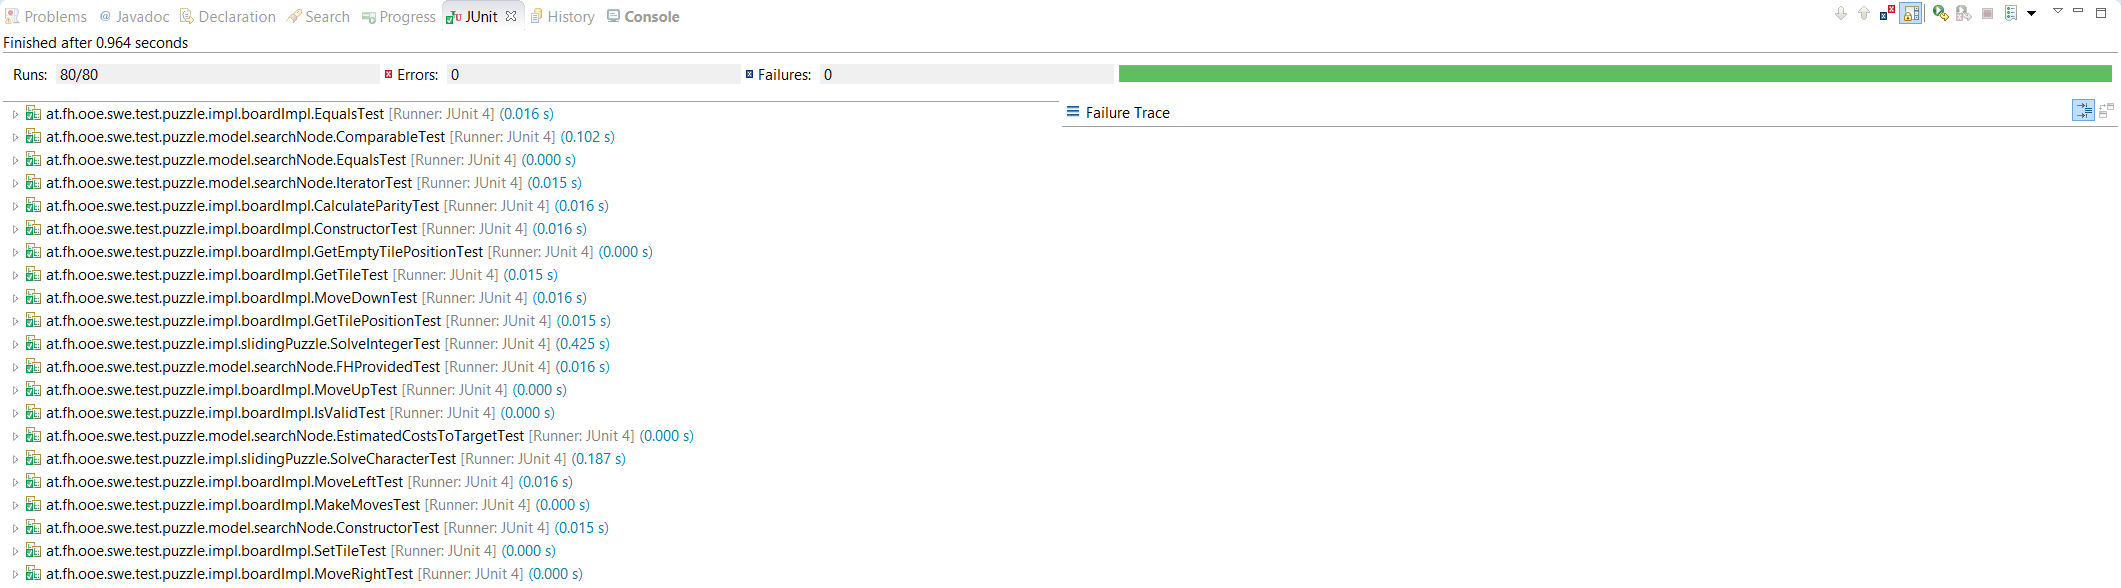
\includegraphics[angle=-90,width=5cm]{\imagesDir/junit_eclipse_all.PNG}
	\caption
	{Diese Abbildung zeigt die JUnit Testresultate im Eclipse}
\end{figure}
\newpage

\begin{figure}[h]
	\centering
	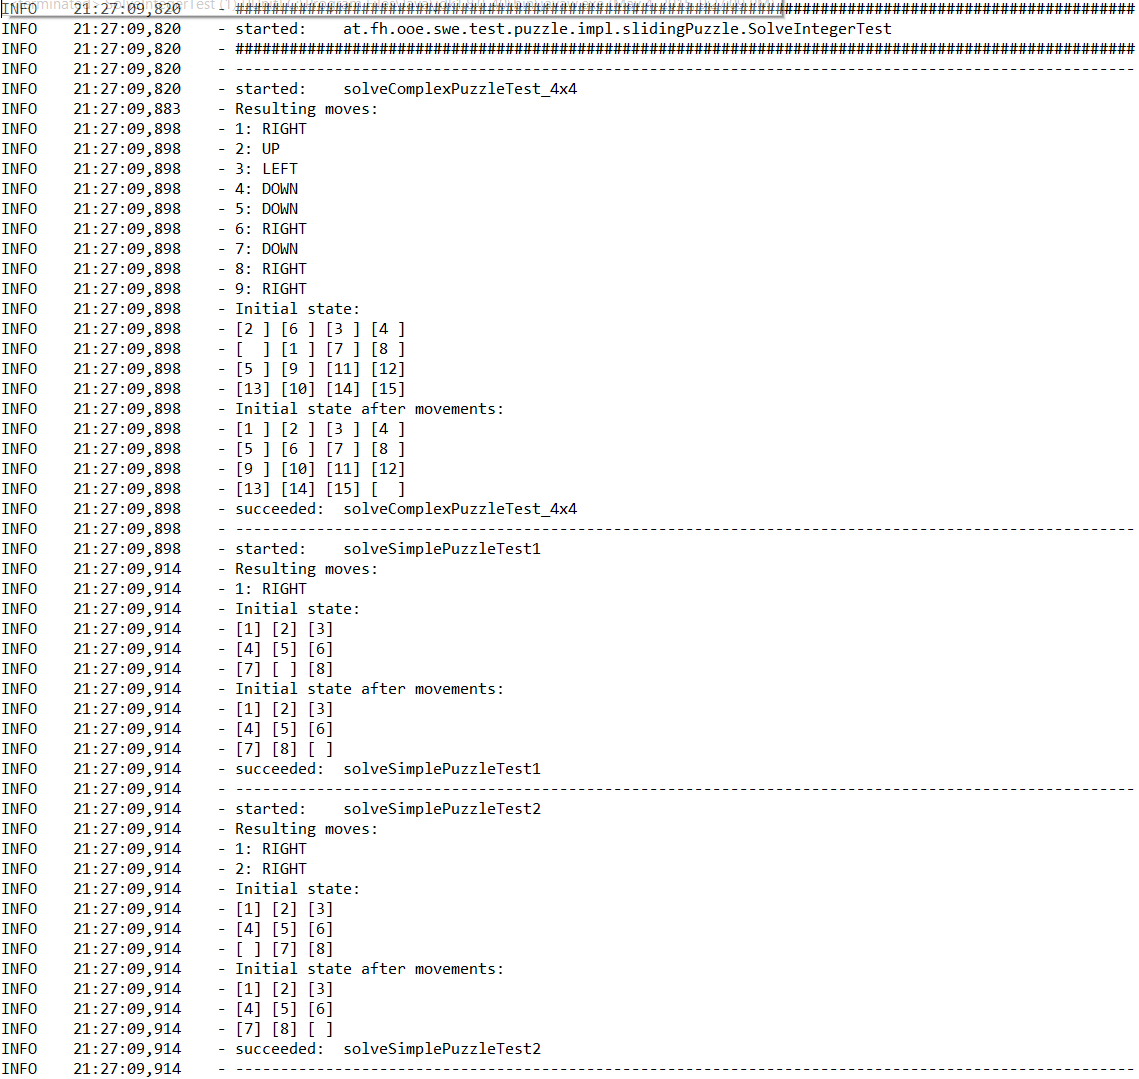
\includegraphics[height=18cm, width=14cm]{\imagesDir/solve_integer_test_1.PNG}
	\caption
	{Diese Abbildung zeigt die Resultate zur Verfügung gestellten Tests mit dem \emph{Integer} Datentyp}
\end{figure}
\newpage

\begin{figure}[h]
	\centering
	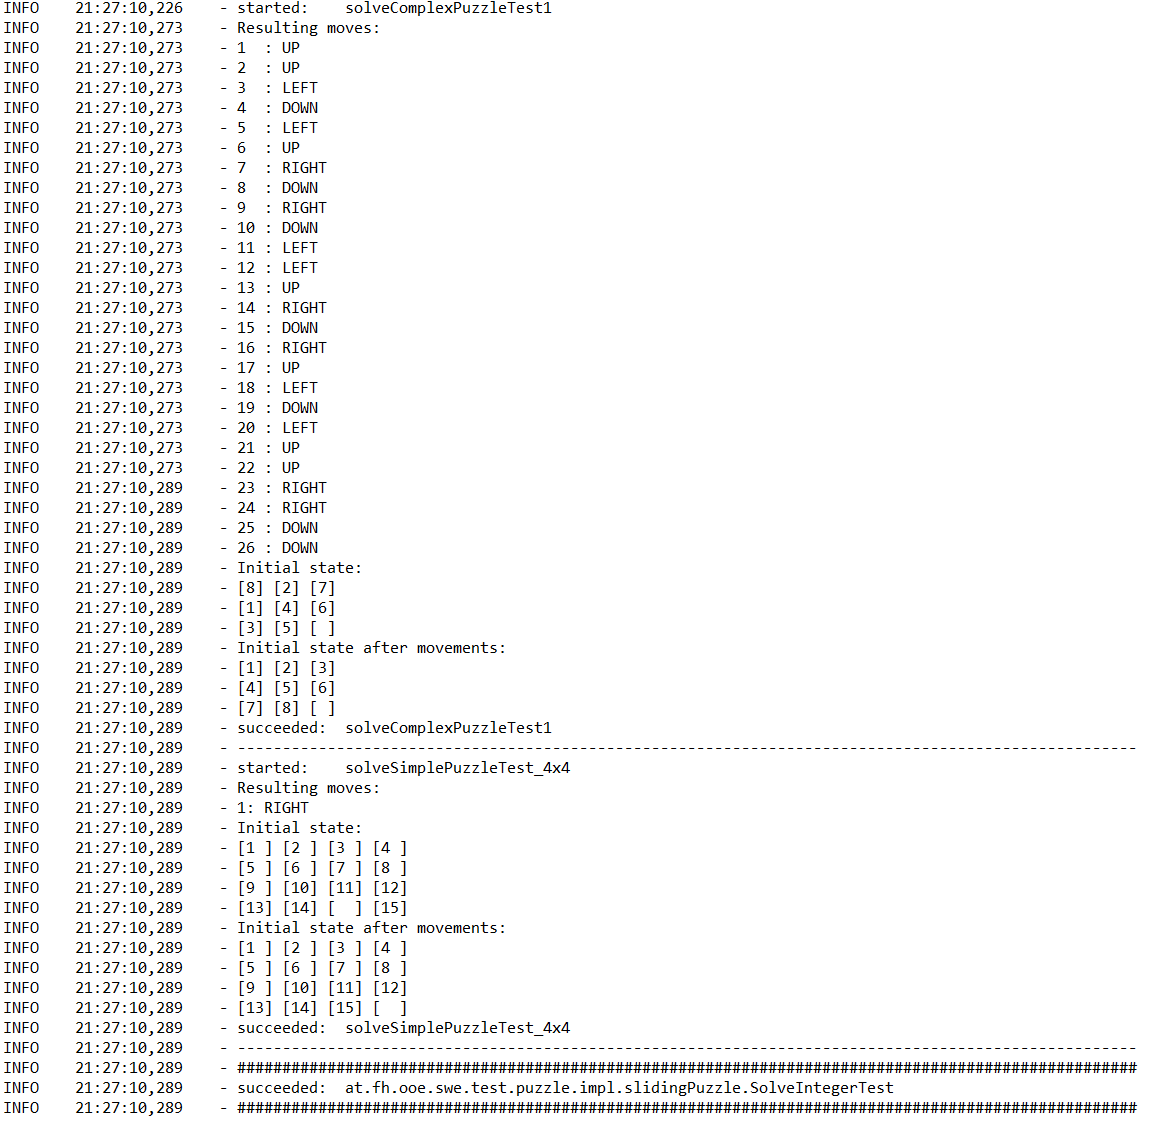
\includegraphics[height=18cm, width=14cm]{\imagesDir/solve_integer_test_2.PNG}
	\caption
	{Diese Abbildung zeigt die Resultate zur Verfügung gestellten Tests mit dem \emph{Integer} Datentyp}
\end{figure}
\newpage

\begin{figure}[h]
	\centering
	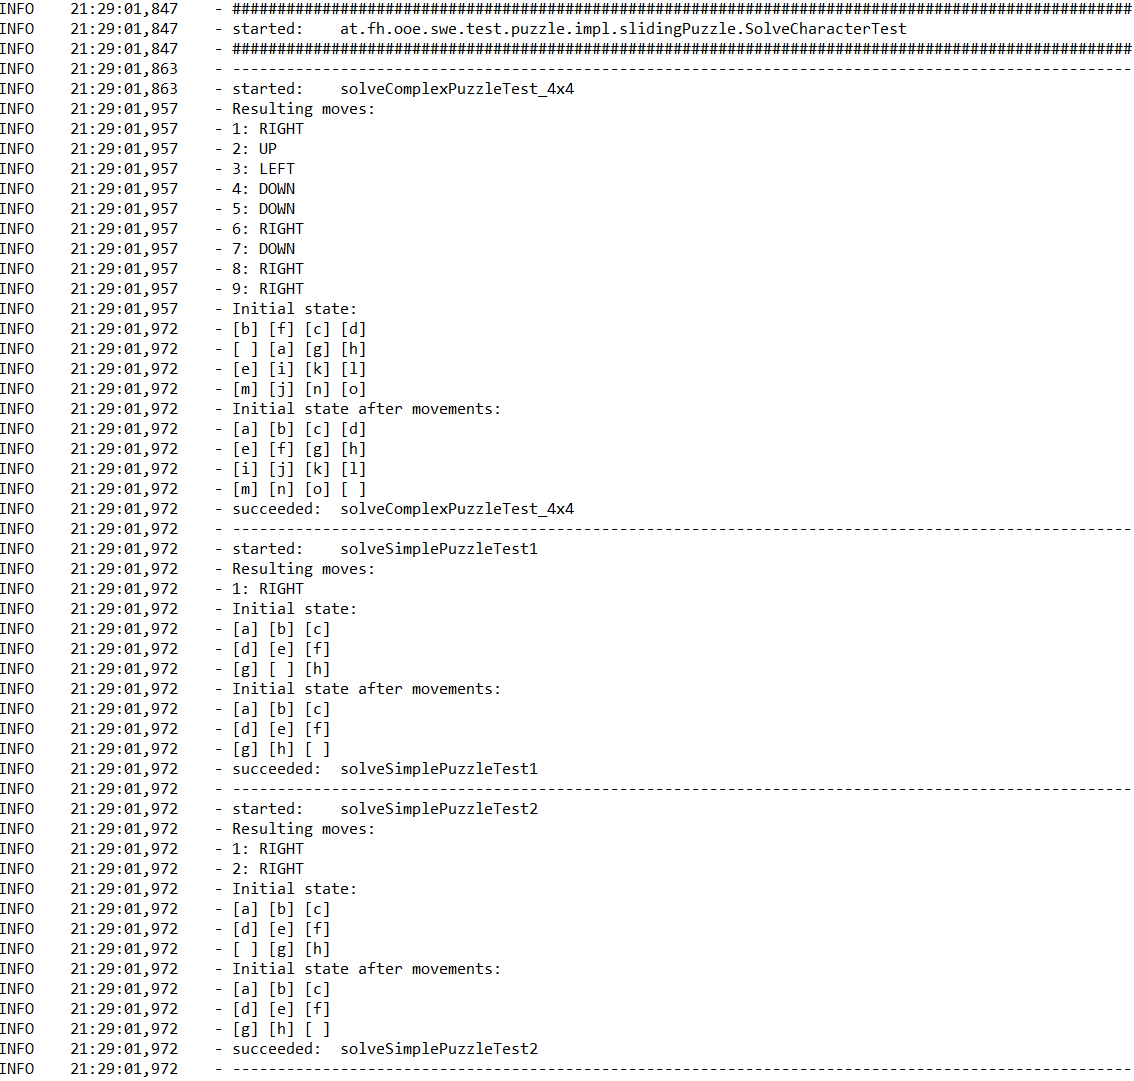
\includegraphics[height=18cm, width=14cm]{\imagesDir/solve_character_test_1.PNG}
	\caption
	{Diese Abbildung zeigt die Resultate zur Verfügung gestellten Tests mit dem \emph{Character} Datentyp}
\end{figure}
\newpage

\begin{figure}[h]
	\centering
	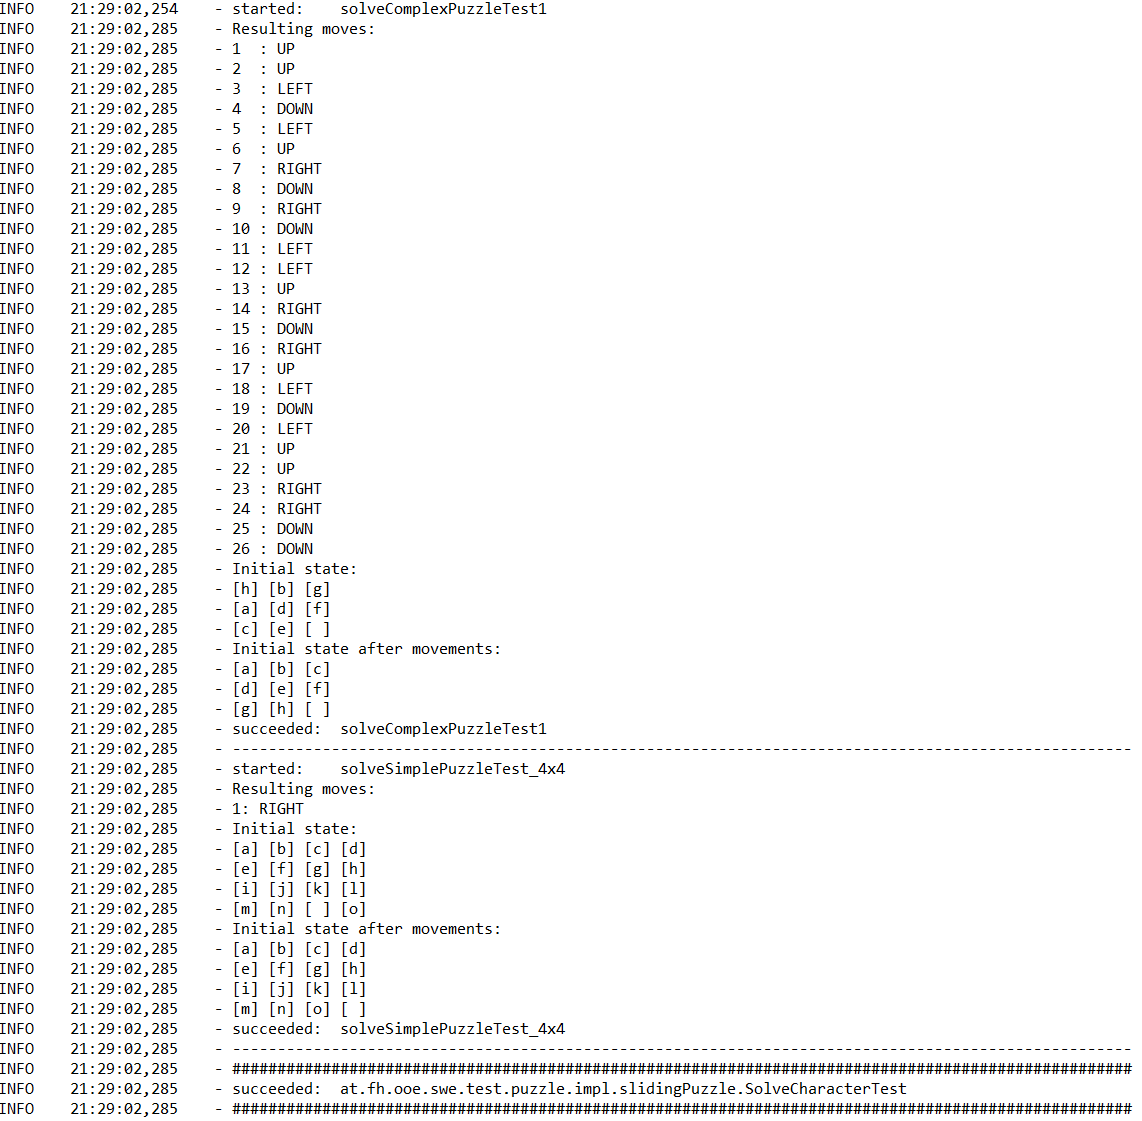
\includegraphics[height=18cm, width=14cm]{\imagesDir/solve_character_test_2.PNG}
	\caption
	{Diese Abbildung zeigt die Resultate zur Verfügung gestellten Tests mit dem \emph{Character} Datentyp}
\end{figure}
\newpage

\begin{figure}[h]
	\centering
	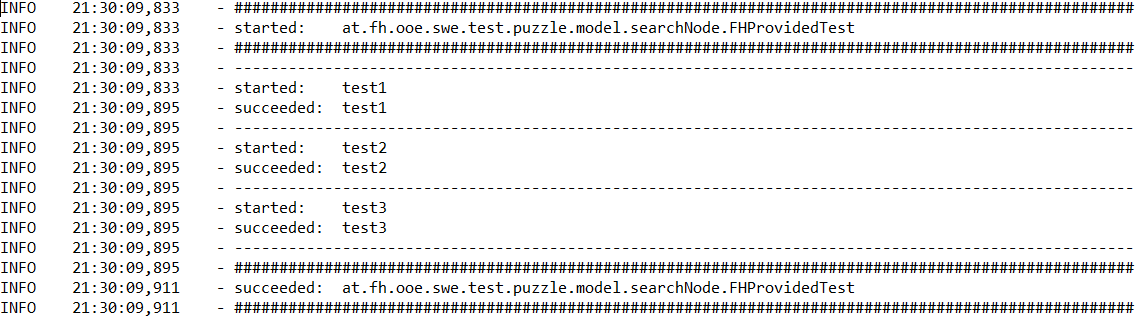
\includegraphics[height=6cm,width=16cm]{\imagesDir/fh_provided_node_test.PNG}
	\caption
	{Diese Abbildung zeigt die Resultate zur Verfügung gestellten Tests für die \inlineJava{SearchNode<T>} angeführt}
\end{figure}
\newpage


\end{document}  